\documentclass{article}

\usepackage[utf8]{inputenc}
\usepackage{caption}
\usepackage{float}
\usepackage{graphicx}

% Change language to change quotation style
\usepackage[english]{babel}
\usepackage{csquotes}

\usepackage{biblatex}
\addbibresource{refs.bib}

\usepackage{hyperref}
\hypersetup{pdfauthor={Cristian Adrián Ontivero}}

\usepackage{adjustbox}
\usepackage{tikz}
\usetikzlibrary{positioning,decorations.pathmorphing,shapes}
\usetikzlibrary{external}
\tikzexternalize[prefix=tikz/, up to date check=md5]

\usepackage{ebproof}
\usepackage{booktabs}
\usepackage{multicol}
% Set items in enumerate environment to letters.
%\usepackage{enumitem}
%\setenumerate[0]{label=(\alph*)}
\usepackage{forest}
\forestset{%
  % Tree following the style of Chiswell & Hodges' Mathematical Logic
  chtree/.style={
    for tree={
      inner sep=1.4pt,
      circle,
      draw,
      s sep'+=20pt,
      fit=band,
    },
  },
  c phantom/.style={draw=none, no edge},
}

\graphicspath{{imgs/}}

\newlength\tindent%
\setlength{\tindent}{\parindent}
\setlength{\parindent}{0pt}
\renewcommand{\indent}{\hspace*{\tindent}}

%These tell TeX which packages to use.
\usepackage{array,epsfig}
\usepackage{amsmath}
\usepackage{amsfonts}
\usepackage{amssymb}
\usepackage{amsxtra}
\usepackage{amsthm}
\usepackage{mathrsfs}

%Pagination stuff.
\setlength{\topmargin}{-.3 in}
\setlength{\oddsidemargin}{0in}
\setlength{\evensidemargin}{0in}
\setlength{\textheight}{9.in}
\setlength{\textwidth}{6.5in}
\pagestyle{empty}

\newcommand{\cit}[2]{\cite[p.~#1~in~][]{#2}}

\begin{document}

Mathematical logic may be considered the outcome of the joining together of
four different lines of thought:
\begin{itemize}
  \item the old logic of Aristotle (and to a much lesser extent, of the Stoics);
  \item the idea of a complete, automatic language for reasoning;
  \item the developments in algebra and geometry after 1825;
  \item and the idea of the parts of mathematics as being systems of deductions.
\end{itemize}

\textbf{Aristotle}:
\begin{itemize}
  \item \textit{Prior Analytics} was the first systematic treatise on formal logic.
  \item Introduced the idea of using variables (letters) in the use of syllogisms.
  \item His logic was the predominant logical method for the next two thousand years.
Immanuel Kant wrote in the introduction of his \textit{Kritik der reinen
Vernunft}:

\enquote{Aristotle invented logic so perfect, that it made no step forward
or backward since then.}

Carl von Prantl\footnote{Philosopher and historian; wrote an important
treatise on the history of logic: \textit{Geschichte der Logik im
Abendlande}, 1855--70, four volumes.} said:

\enquote{any logician after Aristotle who said anything new was confused,
stupid, or perverse.}

\end{itemize}






% In general, page 41 of "The development of logic"
Aristotle anticipates the contraposition of universal affirmative statements:

`In all cases a postulate of this sort should be made: e.g.\ ``If the honorable
is pleasant, what is not pleasant is not honorable, while if the latter is
untrue so is the former''; likewise also ``If what is not pleasant is not
honorable, then what is honorable is pleasant''.'\footnote{\textit{Topica}, ii.
8 (\(113^b22\)).}
\begin{gather*}
  (h \to p) \to (\neg p \to \neg h) \quad \leftrightarrow \quad (\neg p \to \neg h) \to (h \to p)
\end{gather*}

% In general, page 46 of "The development of logic"
% quotes of the Law of Contradiction, and the Law of the Excluded Middle.

% Page 114 Development of logic
Notas del examen
\begin{itemize}
  \item What is a categorical assertion?

  \item What (types?) of categorical assertions are them?

  SaP, SeP, SiP, SoP
  \item What does a categorical assertion for a syllogism need? --> Be
  general (speak of general terms, not singular) and, most importantly, both
  premises must share a middle term, which then does not show on the
  conclusion.

  \item How did aristotle write syllogisms?

  If \(\alpha\) and \(\beta\), then \(\gamma\)

  \item What method did aristotle develop for syllogisms?

  2 methods, an indirect one, and a direct one. The direct one is using
  conversions, the indirect one is giving an informal argument.

\end{itemize}

\newpage
Contributions by The Megarians:
The Liar. \enquote{A man says that he is lying. Is what he says true or false?}.

Crocodile and baby paradox, attributed to Chrysippus by Lucian\footnote{\textit{Vitarum Auctio, 22}}.

According to Philo, all `if-then' statements are true except those that have
a true `if' part and a false `then' part\footnote{Sextus empiricus - Against
the logicians}. This has been the most commonly used if-then in mathematical
logic, named `material implication' by Russell \& Whitehead in their
\textit{Principia Mathematica}. %~\cit{13}{Nid98}.


{% Limit the scope of ny newcommand
\newcommand{\ny}[2]{#1 \\ {\scriptsize #2}}
\begin{figure}[ht] % ’ht’ tells LaTeX to place the figure ’here’ or at the top of the page
\centering % centers the figure
\tikzsetnextfilename{greek-tree}
  \begin{tikzpicture}[node distance=16mm, every node/.style={align=center}]
    \node (soc) {\ny{Socrates}{470 -- 399 BCE}};
    \node[below left=1cm and 15mm of soc] (pla) {\ny{Plato}{42X -- 348/347 BCE}};
    \node[below right=1cm and 15mm of soc] (euc) {\ny{Euclid of Megara}{c. 435 -- c. 365 BCE}};
    \node[below right=5mm and -5mm of euc] (thr) {\ny{Thrasymachus of Corinth}{fl. 4th century BCE}};
    \node[below left=5mm and -5mm of euc] (eub) {\ny{Eubulides of Miletus}{fl. 4th century BCE}}; % Contemporary of Aristotle
    \node[below of=eub] (apo) {\ny{Apollonius Cronus}{fl. 4th century BCE}};
    \node[below=5mm of pla] (ari) {\ny{Aristotle}{384 -- 322 BCE}};
    \node[below=1cm of apo] (dio) {\ny{Diodorus Cronus}{? -- 284 BCE}}; % Contemporary of Stilpo
    \node[below of=dio] (phi) {\ny{Philo the Dialectician}{fl. 300 BCE}};
    \node[below=2.6cm of thr] (sti) {\ny{Stilpo of Megara}{360 -- c. 280 BCE}};
    \node[below of=sti] (zen) {\ny{Zeno of Citium}{334 -- c. 262 BCE}};
    \node[below of=zen] (cle) {\ny{Cleanthes}{330 BCE -- c. 230 BCE}};
    \node[below of=cle] (chr) {\ny{Chrysippus of Soli}{279 -- c. 206 BCE}};

    \draw (soc) edge (pla);
    \draw (soc) edge (euc);
    \draw (euc) edge (thr);
    \draw (thr) edge (sti);
    \draw (euc) edge (eub);
    \draw (eub) edge (apo);
    \draw (apo) edge (dio);
    \draw (dio) edge (zen);
    \draw (pla) edge (ari);
    \draw (dio) edge (phi);
    \draw (phi) edge[dashed] (zen); % Friends, Philo was a kind of "sempai" of Zeno
    \draw (sti) edge (zen);
    \draw (zen) edge (cle);
    \draw (cle) edge (chr);
  \end{tikzpicture}
\caption{Something}\label{fig:my_label}
\end{figure}%
}
Paradoxes contributed by Eubilides
\begin{enumerate}
  \item The liar (pseudomenos).
  \item The Masked Man (enkekalymmenos)
  \item The Electra paradox.
  \item The Heap (sorites) paradox.
  \item The bald man
  \item The Horns (keratines) paradox.
\end{enumerate}

Periods of logic
\begin{enumerate}
  \item Ancient Greece (until 6th century A.D.)
  \item Middle Ages (7th to 11th century)
  \item Scholasticism (11th to 15th)
  \item Modern ``classical'' logic (16th to 19th)
  \item Mathematical logic (mid 19th century onwards)
\end{enumerate}

Square of opposition:
Although the oppositions can be traced back to Aristotle, the drawing is due to Apuleius and Boethius.

\begin{figure}[ht] % ’ht’ tells LaTeX to place the figure ’here’ or at the top of the page
\centering % centers the figure
\tikzsetnextfilename{square-of-oposition}
  \begin{tikzpicture}[node distance=56mm, every node/.style={minimum size=1cm, align=center},
    every label/.style={label distance=-4mm},
    decoration={zigzag,segment length=4,amplitude=.9,
  post=lineto, pre length=6pt, post length=6pt}]
    \node[circle, label=above:Universal affirmative\\All S are P] (sap) {SaP};
    \node[circle, right of=sap, label=above:Universal negative\\No S is P] (sep) {SeP};
    \node[circle, below of=sap, label=below:Some S are P\\Particular affirmative] (sip) {SiP};
    \node[circle, right of=sip, label=below:Some S are not P\\Particular negative] (sop) {SoP};

    \path[<->] (sap) edge node[minimum height=6mm, fill=white, anchor=center, pos=0.5, label=above:\((\uparrow)\)] {\scriptsize contrary} (sep);
    \path[->] (sap) edge node[minimum height=6mm, fill=white, anchor=center, pos=0.5] {\scriptsize subaltern} (sip);

    \path[->] (sep) edge node[minimum height=6mm, fill=white, anchor=center, pos=0.5] {\scriptsize subaltern} (sop);
    \path[<->] (sip) edge node[minimum height=6mm, fill=white, anchor=center, pos=0.5, label=below:\((\lor)\)] {\scriptsize subcontrary} (sop);
    \path[<->] (sip) edge[decorate] (sep);
    \path[<->] (sap) edge[decorate] node[inner sep=1mm, minimum height=0mm, fill=white, anchor=center, pos=0.5, label={[label distance=0mm]above:\((\oplus)\)}] {\scriptsize contradictory} (sop);
  \end{tikzpicture}
\caption{Square of opposition}\label{fig:my_label}
\end{figure}

During the middle ages, the letters a, e, i, and o were used to denote the
different assertions, and come from the latin words \textbf{a}ff\textbf{i}rmo
and n\textbf{e}g\textbf{o}.

The middle ages and modern ``classical'' logic contain, with some notable
exceptions, no innovations.

% From C&H Mathematical Logic
\textbf{Antoine Arnauld}:
\begin{itemize}
  \item His \textit{Port-Royal Logic}, written in 1662 with Pierre Nicole,
  introduced the rule \((\to\text{I})\) as a way of rewriting arguments to
  make them more `beautiful'.
\end{itemize}

\textbf{Leibniz}:
\begin{itemize}
  \item \textit{characteristica universalis}, an alphabet of human thought, a
  universal language which would make all thought transparently clear.
  \item Mechanisation of reasoning
  \item 3rd calculus = first attempt at an abstract mathematics, i.e.\ a
  mathematics not directly concerned with space or numbers.
\end{itemize}

\textbf{Augustus De Morgan}:
\begin{itemize}
  \item First to use the term \textit{Universe of discourse}.
  \item Proposed the name \textit{mathematical logic}.
\end{itemize}

\textbf{Boole}:
\begin{itemize}
  \item His 1847 book \textit{The Mathematical Analysis of Logic, being an
  essay towards a calculus of deductive reasoning} can be said to be the
  start of Mathematical Logic.
\item Wrote \(1-x\) for the complement, and abbreviated it \(\overline{x}\).
This allowed him to write \(x(1-x) = 0\) to represent the principle of
noncontradiction, described by Aristotle and Leibniz as the most fundamental
of all principles.
\item Introduced two special classes: 1, the universe class, and 0, the null class,
for which \(1x = x\) and \(0x = 0\) hold as in ordinary algebra. The universe
class signifies what De Morgan calls the \textit{universe of discourse}.
\item There is one important peculiarity in Boole's system of classes, namely idempotency: \(xx = x\).
Boole notes that this is the distinguishing feature of his calculus.
\item Development, in effect, means turning elective functions into
disjunctive normal form.
\item With ... he gave what we now call a decision procedure. Later ...
realized that Boole's system could be mechanized and presented a machine
doing so.
\end{itemize}

\textbf{Jevons}:
\begin{itemize}
  \item First to make a reasoning machine

\end{itemize}

\textbf{Peano}:


%\cite{MM17}
Provided symbols \(\cap\) for intersection, \(\cup\) for union, \(\in\) for
set membership, \(\exists\) for existential quantification (horizontally
flipped `E'), \(\sim\) for negation, and \reflectbox{C} (flipped `C' for the latin
\textit{consequentia}) used to denote the philonian conditional. This was
later replaced by the horseshoe symbol \(\supset\) in the second volume of
his \textit{Formulaire}, and popularized by Russell \& Whitehead
in their \textit{Principia Mathematica}, where they called it \textit{material conditional}

\textbf{David Hilbert}:
\begin{itemize}
  \item His Göttingen lectures of 1917-1922 were the first systematic
  presentation of first-order logic.
\end{itemize}

\textbf{Charles Sanders Peirce}:
\begin{itemize}
  \item First to use the name ``universal quantifier''.
  \item ``Peirce did for relations what Boole had done for possible subjects
  and predicates: as Boole had turned qualities into classes of the things
  that have the qualities, Peirce turned relations into classes of the groups
  of things between which there are the relations.''
  \item Showed it was possible to give the difinition of all the different
  connectors in terms of \(\uparrow\) (NAND) or \(\downarrow\) (NOR).
\end{itemize}

\textbf{Ernst Schroeder}:
\begin{itemize}
  \item Showed the duality of the laws of algebra.
\end{itemize}

\textbf{Frege}:
\begin{itemize}
  \item TODO
\end{itemize}

\textbf{Cantor}:
\begin{itemize}
  \item In 1874 his paper \textit{Über eine Eigenschaft des Inbegriffes aller
  reellen algebraischen Zahlen} marked the beginning of set theory, and
  showed that there are different kinds of infinity.
  \item In 1878, \textit{Ein Beitrag zur Mannigfaltigkeitslehre} contained
  the notions of a power set, equivalence of sets, and the continuum
  hypothesis.
  \item Debates about set theory are closely related to important questions about logic.
\end{itemize}




``Material implication is a somewhat special and strange sort of implication.
Its attractions are that it is the least strong sort of implication and that
it is generally better than the others for the purposes of mathematics''

{% Limit the scope of ny newcommand
\newcommand{\ny}[2]{#1 \\ {\scriptsize #2}}
\begin{figure}[ht] % ’ht’ tells LaTeX to place the figure ’here’ or at the top of the page
\centering % centers the figure
\tikzsetnextfilename{modern-tree}
  \begin{tikzpicture}[node distance=16mm, every node/.style={align=center}]
    \node (thr) at (-3,3) {\ny{Sir William Hamilton}{1788 -- 1856}};
    \node (euc) at (3, 2) {\ny{Augustus De Morgan}{1806 -- 1871}};
    \node (pla) at (0, 1) {\ny{Boole}{1815 -- 1864}};
    \node (thr) at (-2, -1) {\ny{Gottlob Frege}{1845 -- 1912}};
    \node (thr) at (2, -1) {\ny{Georg Cantor}{1845 -- 1918}};
    \node (thr) at (2, -2) {\ny{Giuseppe Peano}{1858 -- 1932}};
    \node (thr) at (0, -3) {\ny{David Hilbert}{1862 -- 1943}};
    \node (thr) at (0, -4) {\ny{Bertrand Russell}{1872 -- 1970}};
    \node (thr) at (-3, -5) {\ny{L.E.J. Brouwer}{1881 -- 1966}};
    \node (thr) at (0, -6) {\ny{Arend Heyting}{1898 -- 1980}};
  \end{tikzpicture}
\caption{Something}\label{fig:my_label}
\end{figure}%
}

\newpage

%Titus 1:12:13
%\enquote{One of themselves, even a prophet of their own, said, the Cretians
%are alway liars, evil beasts, slow bellies. This witness is true [..]}


\newpage
%\bibliography{refs}
%\bibliographystyle{unsrt}
\printbibliography

\end{document}